\def\fileversion{v1.0} \def\filedate{2018/07/20}
%% Package and Class "uiucthesis2009" for use with LaTeX2e.
\documentclass[edeposit,fullpage,12pt]{uiucthesis2009}
\usepackage[acronym,toc]{glossaries}
\usepackage{graphicx}
%\newacronym{<++>}{<++>}{<++>}
%\newacronym{<++>}{<++>}{<++>}

\newacronym{MTHM}{MTHM}{metric ton of heavy metal}
\newacronym{XS}{XS}{cross-sections}
\newacronym{AO}{AO}{Axial Offset}
\newacronym{PCI}{PCI}{Pellet-Cladding Interaction}
\newacronym{PCMI}{PCMI}{Pellet-Cladding Material Interaction}
\newacronym{lhr}{LHR}{Linear Hear Rate}
\newacronym{SCC}{SCC}{Stress Corrosion Cracking}
\newacronym{MPS}{MPS}{Missing Pellet Surface}

\newacronym{BOC}{BOC}{Beginning of Cycle}
\newacronym{BOL}{BOL}{Beginning of Life}
\newacronym{HZP}{HZP}{Hot Zero Power}
\newacronym{HFP}{HFP}{Hot Full Power}
\newacronym{CASL}{CASL}{Consortium for Advanced Simulation of Light Water Reactors}
\newacronym{IFBA}{IFBA}{Integral Fuel Burnable Absorber}
\newacronym{UMich}{UMich}{University of Michigan}
\newacronym{NCSU}{NCSU}{North Carolina State University}
\newacronym{ORNL}{ORNL}{Oak Ridge National Laboratory}
\newacronym{CMFD}{CMFD}{Coarse Mesh Finite Diference}
\newacronym{INL}{INL}{Idaho National Laboratory}
\newacronym{MOOSE}{MOOSE}{Multiphysics Object Oriented Simulation Environment }
\newacronym{ITC}{ITC}{Isothermal Temperature Coefficient }
\newacronym{CRW}{CRW}{Control Rod Worth}




\newacronym{DOE}{DOE}{Department of Energy}
\newacronym{EPA}{EPA}{Environmental Protection Agency}
\newacronym{EFPD}{EFPD}{Effective Full Power Days}
\newacronym{EOC}{EOC}{End of Cycle}
\newacronym{GWDMT}{GWDMT}{GigaWatt Day per Metric Ton}
\newacronym{DRWM}{DRWM}{Dynamic Rod Worth Measurement}


\newacronym{LWR}{LWR}{Light Water Reactor}
\newacronym{LPPT}{LPPT}{Low Power Physics Tests}

\newacronym{MIT}{MIT}{the Massachusetts Institute of Technology}


\newacronym{NEUP}{NEUP}{Nuclear Energy University Programs}
\newacronym{NPRE}{NPRE}{Department of Nuclear, Plasma, and Radiological Engineering}
\newacronym{NRC}{NRC}{Nuclear Regulatory Commission}

\newacronym{PARCS}{PARCS}{Purdue Advanced Reactor Core Simulator}
\newacronym{PATHS}{PATHS}{PARCS Advanced Thermal Hydraulic Solver}
\newacronym{PWR}{PWR}{Pressurized Water Reactor}
\newacronym{BWR}{BWR}{Boiling Water Reactor}

\newacronym{UOX}{UOX}{uranium oxide}
\newacronym{UQ}{UQ}{uncertainty quantification}
\newacronym{US}{U.S.}{United States}
\newacronym{UIUC}{UIUC}{University of Illinois at Urbana-Champaign}
\newacronym{VV}{V\&V}{verification and validation}
\newacronym{VERA}{VERA}{Virtual Enviromnment for Reactor Analysis}
\newacronym{VERACS}{VERA-CS}{VERA Core Simulator}
\newacronym{BEAVRS}{BEAVRS}{Benchmark for Evaluation And Validation of Reactor Simulations}
\newacronym{BW}{B\&W-1484}{Babcock and Wilcox critical experiments Series 1484}



\begin{document}

\title{Investigation of Pellet Clad Interaction during Load-Follow\\
       Operation in a Pressurized Water Reactor using VERA-CS}
\author{Daniel John O'Grady}
\department{Nuclear, Plasma, and Radiological Engineering}
\schools{B.S., University of Illinois at Urbana-Champaign, 2017}
\msthesis
\advisor{Tomasz Kozlowski}
\degreeyear{2018}
\committee{Professor Tomasz Kozloski, Advisor}%\\Professor Katherine Huff}
\maketitle

\frontmatter

%% Create an abstract that can also be used for the ProQuest abstract.
%% Note that ProQuest truncates their abstracts at 350 words.
\begin{abstract}
This is a comprehensive study of caffeine consumption by graduate
students at the University of Illinois who are in the very final
stages of completing their doctoral degrees. A study group of six
hundred doctoral students\ldots.
\end{abstract}

%% Create a dedication in italics with no heading, centered vertically
%% on the page.
\begin{dedication}
To Father and Mother.
\end{dedication}

%% Create an Acknowledgements page, many departments require you to
%% include funding support in this.
\chapter*{Acknowledgments}

This project would not have been possible without the support of
many people. Many thanks to my adviser, Lawrence T. Strongarm, who
read my numerous revisions and helped make some sense of the
confusion. Also thanks to my committee members, Reginald Bottoms,
Karin Vegas, and Cindy Willy, who offered guidance and support.
Thanks to the University of Illinois Graduate College for awarding
me a Dissertation Completion Fellowship, providing me with the
financial means to complete this project. And finally, thanks to
my husband, parents, and numerous friends who endured this long
process with me, always offering support and love.

%% The thesis format requires the Table of Contents to come
%% before any other major sections, all of these sections after
%% the Table of Contents must be listed therein (i.e., use \chapter,
%% not \chapter*).  Common sections to have between the Table of
%% Contents and the main text are:
%%
%% List of Tables
%% List of Figures
%% List Symbols and/or Abbreviations
%% etc.

\tableofcontents
\listoftables
\listoffigures

%% Create a List of Abbreviations. The left column
%% is 1 inch wide and left-justified
\chapter{List of Abbreviations}

\begin{symbollist*}
\item[CA] Caffeine Addict.
\item[CD] Coffee Drinker.
\end{symbollist*}

%% Create a List of Symbols. The left column
%% is 0.7 inch wide and centered
\chapter{List of Symbols}

\begin{symbollist}[0.7in]
\item[$\tau$] Time taken to drink one cup of coffee.
\item[$\mu$g] Micrograms (of caffeine, generally).
\end{symbollist}

\mainmatter

%%%%%%%%%%%%%%%%%%%%%%%%%%%%%%%%%%%%%%%%%%%%%%%%%%%%%%%%%
%%%%%%%%%%%%%%%%%%%%%%%%%%%%%%%%%%%%%%%%%%%%%%%%%%%%%%%%%
\chapter{Introduction}
%%%%%%%%%%%%%%%%%%%%%%%%%%%%%%%%%%%%%%%%%%%%%%%%%%%%%%%%%
%%%%%%%%%%%%%%%%%%%%%%%%%%%%%%%%%%%%%%%%%%%%%%%%%%%%%%%%%

In the \gls{US}, nuclear power generation has high fixed costs and low variable costs. 
As a result, utilities have traditionally sought to operate nuclear stations at full power from \gls{BOC} to \gls{EOC}. 
More recently, the deregulation of the energy market and the emergence of intermittent renewable energy sources have caused load-follow operation to become a more attractive option for nuclear generation. 

The deregulation of the energy market has forced utilities to compete against each other to sell electricity within a region.
The beneficiary of this competition are the customers, who are guaranteed fair prices for electricity and will not be footing the bill for an inefficient/uneconomical utility project. %need citation
Nuclear stations have typically been able to economically compete within deregulated markets because the typical plant lifetime of at least 20 years allows owners to spread out the fixed costs.
Recently, the low price of natural gas and government subsidized renewable energy sources, such as wind and solar, have made nuclear stations appear uneconomic.   

%%%%%%%%%%%%%%%%%%%%%%%%%%%%%%%%%%%%%%%%%%%%%%%%%%%%%%%%%
\section{Background and Motivation}
%%%%%%%%%%%%%%%%%%%%%%%%%%%%%%%%%%%%%%%%%%%%%%%%%%%%%%%%%

In 2016, the \gls{US} had approximately 7\% of its total electricity generation coming from wind and solar power \cite{u.s_energy_information_administration_electricity_2016}. 
This share is likely to increase as the \gls{US} continues to move away from fossil fuels and towards a "greener" energy future.
As a result of this increase, in combination with the deregulation of the energy market, the price of electricity has become volatile. 
At certain times, the price of selling electricity within a region can even become negative, due a sudden increase in renewable energy output and a low market demand \cite{paraschiv_impact_2014}. 
In some areas, negative electricity prices are further increased due to the fact that large generating facilities would rather sell at a loss to avoid decreasing their power level. 
This preference is caused by the high capital cost and relatively low variable costs of large generating facilities \cite{lokhov_load-following_2011}.

Nuclear stations are typically one of these large generating facilities.
As a result of the large construction costs and the fixed number of staff members that must be on site at all times, most utilities prefer to keep a reactor at full power, as it is easiest to maintain constant power. 
If instead of remaining at full power, a nuclear station operated in load-following mode, could this increase the efficiency of the plant?
During load-follow operation, a nuclear station will vary its power output in response to the anticipated demand to better suit the market needs, stabilizing the price of electricity.
Theoretically, the current operating plants were all designed with the maneuverability to respond to such change in demand \cite{lokhov_technical_2011}.
In fact, many of the reactors in France already participate in load-following maneuvers with the help of grey control rods \cite{lokhov_technical_2011}.
Grey control rods are similar to standard \gls{PWR} control rods but have significantly less rod worth \cite{yousefpour_improvement_2000}.
The low rod worth allows them to be used for reactivity control without putting significant stress on the surrounding fuel. 
In the \gls{US}, grey rods are not present in \gls{PWR}, increasing the complexity of load-follow operation \cite{lokhov_technical_2011}.
  
To participate in load-follow operation in the \gls{US}, a \gls{PWR} can use the critical boron concentration to modify the power level while making minor control rod insertion to manage the core \gls{AO} \cite{lokhov_technical_2011}.  
This practice, in addition to the response of the local Xenon concentrations, can lead to significant changes in local pin powers throughout the core.
Changes in local power can cause fuel to swell or contract, due to thermal expansion \cite{gartner_power_1984}. %need citation
If a utility chooses to ramp down the reactor during times of low demand, or high supply, the fuel pellets will contract.
When the decision is made to return the reactor back to full power, the rate at which the power can be increased is limited by the thermal expansion of the fuel pellets \cite{gartner_power_1984}.
A sudden expansion of the fuel pellet has the potential to exert additional stress on the cladding, commonly referred to as \gls{PCMI}.
\gls{PCMI} can lead to fuel failure by \gls{PCI}, and has been extensively investigated since the early 1970s.

\gls{PCI} induced fuel failure is the result of \gls{PCMI} and environmental contributions.
\gls{PCMI} is best described as the material interaction at the pellet-clad interface which creates a stress state on the fuel cladding \cite{kennard_pci_2016}.
This material interaction is commonly caused by the thermal expansion of $UO_2$ fuel pellets during changes in power.
%Oguma \cite{oguma_cracking_1983} found that a fuel pellets radius changes exponentially with its \gls{lhr}, thus large changes in power cause the fuel pellet to contact and strain the cladding.
In addition to the mechanical stress being exerted on the cladding, environmental contributions, chemical or geometrical in nature, have an adverse effect on the claddings integrity.
Chemical environments arise from the release of fission products from the fuel pellet.
Iodine and cadmium-in-cesium are considered to be the most corrosive fission products released from the pellet. %need citation
In the presence of prolonged \gls{PCMI}, the corrosive chemical environment causes inter granular crack propagation, or \gls{SCC}, through the zircaloy based cladding.
This type of cladding failure is commonly referred to as \gls{PCI}-\gls{SCC}, or "classical \gls{PCI}."

%Go into more detail on hoop stress and $PCMI$
%Include a photo of what hoop stress is, describe the harsh environment of a fuel pellet

Geometric contributions to \gls{PCI} are a result of irregularities in the fuel pellet shape.
Typical \gls{LWR} fuel pellets are ceramic $UO_2$ cylinder with a height of approximately 1 cm and dishes and chamfers on the top and bottom of the pellet.
Hundreds of these pellets are stacked into a single fuel, with approximately 60,000 fuel rods in a \gls{LWR} core.
The shear quantity of fuel pellets ordered by a utility makes it impossible for a fuel vendor to ensure no pellet has a defect.
The most common defect is a \gls{MPS}, where part of the fuel pellet has chipped off during manufacturing.
This chip causes asymmetric expansion of the pellet during power maneuvers leading to an increased local stress on the fuel cladding. 
If this stress exceeds the yield stress of the cladding, brittle failure is likely to occur.
This type of cladding failure is commonly referred to as \gls{PCI}-\gls{MPS}, as the missing surface is the critical feature in causing the failure.


%%%%%%%%%%%%%%%%%%%%%%%%%%%%%%%%%%%%%%%%%%%%%%%%%%%%%%%%%
\section{Literature Review}
%%%%%%%%%%%%%%%%%%%%%%%%%%%%%%%%%%%%%%%%%%%%%%%%%%%%%%%%%

In the early 1970's a string of fuel failures in \gls{BWR} led to the first classification of \gls{PCI} induced fuel failure.  
Shortly after, \gls{PCI} induced fuel failures were found in \gls{PWR} and determined to be an inherent problem in \gls{LWR} zircaloy based fuels. %Find citation
The majority of these failures were observed during or shortly after power maneuvers from hot zero power.
To reduce the risk of failure, fuel manufactures made design modifications and began to provide power ramping guidelines \cite{kennard_pci_2016}.
These ramp guideline were particularly conservative and focused primarily on \gls{BOC} power ramps. 
Since then, \gls{PCI} has been extensively studied in order to increase the efficiency of reactor start-up and minimize the number of fuel failures.
%In order to extend the results of these studies to load follow operation, the driving forces of \gls{PCI} must be analyzed to determine their significance mid cycle power ramps.
 
%%%%%%
%First Paper
%%%%%%
Cox \cite{cox_pellet-clad_1990} performed an extensive review of the work done on zircaloy fuel failures caused by \gls{PCI} up to 1972.
He begins by outlining all of the factors that can contribute to \gls{PCI} failures.
The most significant factor in \gls{PCI} is the geometry of the fuel pellet. 
The strain on the cladding is determined by
\begin{enumerate}
\item manufactured gap size
\item shape of the fuel pellet
\item effect of the chamfers and groves.
\end{enumerate} 
In addition to manufactured defects in the fuel pellets, he highlights that ceramic $UO_2$ also experiences a number of geometric changes as a function of radiation exposure and temperature/power level.
These changes include but are not limited to fuel pellet  densification, cracking, relocation, and thermal expansion. 
Pellet cracking and relocation contribute significantly to strain experience by the cladding due to the differential movement of the pellets  relative to one another.
This differential movement is further intensified  by the locking of crack edges into cracks with the cladding and the local coefficient of friction between the pellet/cladding.
At high exposure the coefficient of friction can approach infinity as fission products have escaped the fuel pellet and have cemented the pellet to the cladding. 

In addition to the contribution the fuel pellet geometry has on the local strain, the cladding material and geometry determine how the cladding will respond to the strain.
The wall thickness to diameter ratio and creep rate of the cladding effect the magnitude of the initial stress and the rate at which the stress decays.
The total stress imposed on the cladding a function of maximum power, which determines the total expansion of the fuel pellet, and the change in power during a power ramp, which determines the increment in cladding strain.
Cox goes on to highlight the importance of a corrosive agent at causing \gls{PCI}, noting that Iodine and Cadmium-in-Cesium are the largest contributors to the corrosive environment at the cladding surface.
To minimize the risk of \gls{PCI}, Cox emphasized the importance of fuel conditioning or holds at intermediate power during large power ramps.
Fuel conditioning allows the cladding to relieve some of the stress experienced during the initial ramp while also influencing the chemical environment.
Together these effects reduce the propagation of cracks through the cladding surfaces.
%%%%%%

%%%%%%
%Second Paper
%%%%%%
Jernkvist \cite{jernkvist_model_1995} developed a model for predicting \gls{PCI} induced fuel failure based on crack initiation and growth.
Jernkvist model stressed three key parameters involved in \gls{PCI},
\begin{itemize} 
\item cladding stress and strain are extremely localized, 
\item fuel rod failure due to \gls{PCI} is normally a result of a sudden power increase 
\item \gls{PCI} induced failure within a reactor core shows strong variability.
\end{itemize}
Jernkvist recognized that crack propagation occurs in two stages, slow intergranular propagation followed by rapid transgranular crack growth.
Due to the presence of internal flaws within the cladding, Jernkvist neglected the intergranular process.
In order to account for the stochastic nature of \gls{PCI} in reactor cores, a probabilistic treatment of the initial crack size was used.
The crack propagation velocity was then determined by the stress, temperature, and iodine concentration at the tip of the crack.
Using a finite element solver, Jernkvist calculated the stress at the tip of the crack.
If the stress was greater than the iodine stress corrosion crack threshold, the velocity was determined using a correlation requiring the temperature and iodine concentration.
To simplify the determination of the iodine concentration, a correlation was used based on the power and fuel burnup.
It was then assumed that all of the iodine collects at the pellet-pellet interface and radial pellet cracks.

With the velocity of the crack propagation known the time to cladding failure can be calculated.
Using an artificial power history, Jernkvist provides an example where the coefficient of friction is varied for the pellet-clad interface.
At sufficiently high coefficients of friction, the local stress on the cladding is high enough to grow the crack through the cladding.
This demonstration shows the importance of accurately determining the stress within the cladding when trying to predict cladding failure.
Additionally, it highlights the need for a coupled multiphysics approach as the coefficient of friction at the pellet-clad interface is a function of temperature and burnup.
%%%%%%

%%%%%%
%Third Paper
%%%%%%
One of the computational codes that attempts to incorporate this multiphysics approach is FALCON. %Need citation
FALCON is a fully coupled, thermo-mechanical, two dimensional finite element computer code being developed by \gls{EPRI}.
Building on the material properties provided in MATPRO, FALCON has the ability to simulate $UO_2$ pellet relocation, fission gas release and zircaloy cladding thermal creep.

FALCON has been extensively benchmarked and is commonly used by contractors and utilities to mitigate the risk of \gls{PCI} induced fuel failure.
Lyon et al. \cite{lyon_pci_2009} used FALCON in order to determine a criteria for mitigating \gls{PCI} induced fuel failure during power ramps.
The authors point out that power ramp rate restrictions, which are normally set by fuel vendors, and power conditioning, the practice of taking intermediate holds at constant power, are not reliable at mitigating the risk of \gls{PCI}. 
Rather, these practices lead to restrictive constraints on plant operation.

Another criteria that is commonly suggested is the implementation of a stress based threshold.
The authors argue that stress based thresholds are unable to distinguish between failed and non failed fuel rods, leading to a conservative threshold when applied to power maneuvers.
In its place they propose a mechanistic approach that incorporates \gls{PCMI} and \gls{SCC} based cumulative damage.

Similar to Jernkavist,  Lyon et al. recognized that cladding failure due to \gls{SCC} occurs in two stages, crack incubation and crack propagation.
The \gls{CDI} model in FALCON accounts for both of these stages using a cumulative damage process, where damage accumulation is linear with time.
This allows the damage fraction, $D$, to be defined as 
\begin{equation}\label{eqn:paper_3_eqn_1}
D = \int \frac{dt}{\bar{t}}
\end{equation}
where $\bar{t}$ is the time-to-failure.
The time-to-failure of a material is normally measured in an \gls{SCC} out-of-pile test and is defined as
\begin{equation}
\bar{t} = f(\sigma,\sigma_y,\sigma_{ref},B,T)
\end{equation}
where $\sigma$ is the applied hoop stress, $\sigma_y$ is the materials yield strength, $\sigma_{ref}$ is burnup dependent function, $B$ is the burnup of the fuel, and $T$ is the temperature.
It is important to note that Equation \ref{eqn:paper_3_eqn_1} only applies to a single power maneuver, therefore $D$ must be summed over all power maneuvers. 
Experience has shown that $D$ exhibits logarithmic behavior with stress, therefore it should be interpreted probabilistically, where $D=1$ represents a 50\% failure probability while $D=0.1$ and $D=10$ imply a $<5$\% and $>59$\% failure probability.
In order to account for the possibility that cladding stress can drop below the \gls{SCC} threshold during ramps and environmental difference between in-pile and out-of-pile fuel rods, an adjustable single valued parameter $\beta$ is introduced to the \gls{CDI} model. 
\begin{equation}
D = \sum \frac{\delta t_i}{\beta \bar{t_i}}
\end{equation}

In order to demonstrate the accuracy of a \gls{CDI} based criteria, Lyon et al. simulated 14 fuel rods from the Studsvik Over Ramp, Super Ramp and Trans Ramp IV program, as well as, rods from a CEA/OSIRIS ramp program using FALCON.
These simulations were broken into three parts, first a steady state two dimensional, R-Z, depletion simulation is performed using the power histories of each rod.
The results of these simulations are then used as the initial condition for transient R-Z simulations of the different power ramps under investigation.
Finally, an R-$\theta$ model containing discrete fuel cracks is created for the axial location which experienced the highest R-Z hoop stress.
This simulation provides the fuel pins maximum clad hoop stress and \gls{CDI} which can then be used to determine a threshold criteria.

After validating the steady state simulations against \gls{PIE} measurements, Lyon et al. performed the transient analysis for all of the fuel rods. 
The power history of fuel rod Q11/1, along with the maximum cladding hoop stress and \gls{CDI} are shown in Figure \ref{fig:paper_3_res}.
It is observed that the \gls{CDI} only changes during sharp power ramps while the hoop stress more closely follows the power profile.

Using the results of all 14 fuel rods, the authors established a statistical failure criteria using both hoop stress and \gls{CDI}.
A 550 MPa maximum clad hoop stress  and a \gls{CDI} of 5.85 were determined to signify a 50\% chance of rod failure.
Using the 50\% chance as a hard cut off between non-failed and failed rods, the authors evaluated how each of the criteria performed using the 14 fuel rods.
The peak stress was able to corrected predict the behavior of eight out of the 14 fuel rods while the \gls{CDI} predicted the behavior of 13 out of the 14 rods.
Although this work does show the superiority of a \gls{CDI} based criteria, the training set and validation set are considerably small.
Additionally, the power ramps used during the test program are extreme and are unlikely to be performed during standard operation.
As a result further validation is needed for a \gls{CDI} based criteria.
 
\begin{figure}
\begin{tabular}{cc}
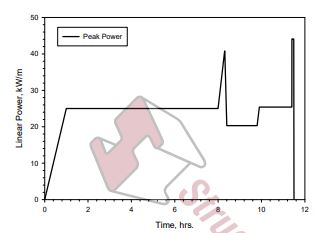
\includegraphics[width=0.5\linewidth]{./Figures/lyon_image_6.JPG} & 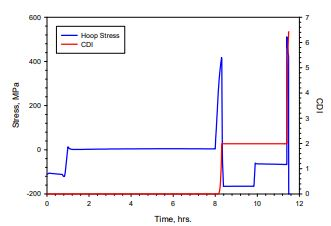
\includegraphics[width=0.5\linewidth]{./Figures/lyon_image_7.JPG}
\end{tabular}
\caption{The Power history (left), Falcon predicted hoop stress and Falcon predicted CDI (right) for Q11/1 of the Studsvik ramp program \cite{lyon_pci_2009}}
\label{fig:paper_3_res}
\end{figure}
%%%%%%


%%%%%%
%Fourth Paper
%%%%%%
Similar to Lyon et al., Capps et al. \cite{capps_pci_2017} used BISON to investigate fuel rods that failed during the start up ramp of a commercial \gls{PWR}.
Before Capps et al. could begin applying failure thresholds to fuel rods under investigation, the thresholds needed to be determined using BISON as the FALCON ones would not apply.
To do so, the Studsvik ramp tests were implemented in BISON using a four step process.
The first three steps follow the same methodology used by Lyon et al, R-Z depletion followed by an R-Z fuel performance calculation, ending with a R-$\theta$ fuel performance simulation at the axial location with the highest hoop stress.
The fourth step, which is unique to BISON, is a three dimensional R-$\theta$-Z fuel performance simulation of the entire rod.
Although BISON is capable of computing \gls{CDI}, the authors only report the failure thresholds based on the peak cladding hoop stress.
The results of both the R-$\theta$ and the three dimensional simulations were consistent with the results presented by Lyon et al.
The authors observed that the hoop stress calculated in the three dimensional study was consistently higher than the hoop stress from the R-$\theta$ study.
This signifies the importance the pellet's height has on the cladding stress.
Although the three dimensional stress was elevated no clear cutoff was observed to distinguish the failed fuel rods from the intact fuel rods.
For this reason, a statistical approach was developed for both the R-$\theta$ and the three dimensional simulations.

Using the same four step methodology, the authors performed fuel performance simulations on several fuel rods from the commercial \gls{PWR}.
Two different cycle startup ramps were investigated; the first cycle contained three failed fuel rods and the second contained a single failed fuel rod.
The power histories for the R-Z depletion were provided by Westinghouse and are assumed to be from a nodal core simulator.
Before analyzing any of the BISON results the authors observed important characteristics from the fuel rods power histories.
Two of the failed rods in the first cycle were exposed to aggressive irradiation linear heat rates during their initial cycles.
This led to the rods accumulating high burnups and the closing of the gap.
The third failed rod saw a significant increase in its linear heat rate after its initial cycle.
As noted in the previous works, these characteristics are strong indicators for potential \gls{PCI} induced fuel failure. 

In order to account for the change in cladding material, zirc4 in the Studsvik tests, zirlo in the commercial reactor, Capps et al. scaled the thresholds to 395 MPa for the R-$\theta$ and 446 MPa for the three dimensional predictions.
The peak cladding hoop stress for all three of the failed rods was predicted to be below the threshold in both simulations.
Additionally, two of the non-failed rods that were simulated were predicted to have peak cladding hoop stress above the threshold. 
This led the authors to conclude that "classical" \gls{PCI} could not be the cause of the failure.
After introducing a \gls{MPS} to each of the simulated rods, all peak cladding hoop stresses fell above the 5\% failure threshold.
Furthermore, one of the fuel rods was confirmed to have a \gls{MPS} during a \gls{PIE}, confirming the results of the simulation.

In order to reduce the probability of \gls{PCI} induced failure, classic and \gls{MPS} induced, Exelon implemented strict power ramp rates and began to introduce power holds during return to full power ramps.%Insert MPS sensitivity study details 
Capps et al. investigated the effects of these restrictions on the cladding hoop stress and found that they could reduce the peak stress by approximately 50 MPa.
Even with the reduction in failure risk associated with the decrease in hoop stress, fuel failure was still experienced during the initial power maneuver.
This suggests that pellet defects are a major contributor to fuel failure during power maneuvers. 
Using the restrictive power history developed by Exelon, Capps et al. performed a sensitivity study on the maximum clad hoop stress as a function of \gls{MPS} length.
Westinghouse specifications limit the dimension of a \gls{MPS} to 60 mils, but lengths up to 125 mils have been observed during \gls{PIE}.
For this reason, \gls{MPS} with lengths ranging from 60 to 140 mils were simulated using 2D and 3D BISON simulations. 
The hoop stress resulting from a \gls{MPS} is a result of pellet thermal expansion. 
As the pellet expands the missing face does not exert an outward force on the cladding, causing the cladding to bend at the edges of the \gls{MPS}.
In 2D simulations the hoop stress increases linearly with the length of the \gls{MPS}, with a widths of 110 mils increasing the probability of failure to 50\%.
These simulations are inherently flawed as adiabatic boundary conditions are applied to the top and bottom the fuel slice, resulting in the limitation that heat must be conducted radially.
As the missing pellet surface grows, the heat transfer across the gap degrades leading to an increase in pellet temperature.
This increase in temperature causes the pellet to continue to swell, exerting additional pressure on the cladding.

In reality, the heat will flow in the direction of the least resistance, i.e. axial conduction will compensate for the reduction in heat transfer across the gap.
This effect is captured in the 3D simulations, which show miniscule changes in the maximum fuel temperature as a function of \gls{MPS} width.
A \gls{MPS} width of 100 mils was found to result in a 50\% chance of fuel failure during the restrictive power ramps.
Unfortunately, the 3D simulations were performed using an infinite coefficient of friction between the pellet and cladding, causing elevated stresses in the cladding.
%%%%%%

%%%%%%
%Fifth Paper
%%%%%%

In order to more comprehensively understand the effect pellet defects have on the cladding, Capps et al. studied the individual effects of fuel cracks and \gls{MPS}.
The stress on the cladding caused by pellet cracks is a function of the crack length and the spacing in between cracks.
As the crack spacing increases within the fuel pellet the number of cracks within the pellet decreases.
This cause the opening of a single pellet to increase, which increases the tangential stress on the cladding at the cracks opening.
It is typically found that commercial fuel has six to ten radial cracks, which helps to reduce the stress on the cladding.

The length of a fuel pellet crack characterizes the compliance of the fuel pellet to its manufactured cylindrical shape.
As the crack length increases, the fuel pellet is less compliant and creates a shear stress on the cladding.
Capps et al. found that the shear stress exerted begins to saturate when the crack length approaches 50\% of the pellet radius.
Although the stress on the cladding has saturated, the stress at the tip of the crack is larger than the  at a length of 50\%. %Need word here
This suggests that the crack will continue to propagate until it has reached approximately 70\% of the pellet radius.

In most cases, \gls{MPS} are accompanied by cracks.
This makes it necessary to incorporate pellet cracks when determining the effect of \gls{MPS}.
Unlike pellet cracks \gls{MPS} cause hoop stresses within the clad through bending forces.
This hoop stress shows a saturation as the \gls{MPS}width increases.
In addition to the width of the \gls{MPS}, the shape of the defect has a strong effect the maximum hoop stress.
It is typical to simulate \gls{MPS} as flat defects, although it is more likely they will be concave in shape. 
This concavity further reduces the pellet-gap conductivity causing a rise in the fuel temperature and an increase in the maximum hoop stress.

Although 2D simulations are useful in determining the effect of fuel cracks and \gls{MPS}, they are inherently flawed as much of the axial effects are lost in the boundary conditions.
In addition to the loss of heat transfer in the axial direction, structural support is not taken into consideration as the \gls{MPS} has an infinite hight.
Unfortunately three dimensional contact makes the simulation of cracks and \gls{MPS} difficult, and prohibits a full length fuel rod from being simulated in three dimension. 
To work around this, Capps et al. simulated a stack of five discrete fuel pellets with a \gls{MPS} included in the center fuel pellet.
The results of the three dimensional study showed that axial contributions reduce the maximum cladding hoop stress by 7 to 15 \%.
Although this reduction is significant, the trends observed in the two dimensional studies did not change.
Therefore, fuel performance studies can be conducted in two dimensions as long as the thresholds for stress were determined using consistent two dimensional studies.

%%%%%%

%%%%%%
%Sixth Paper
%%%%%%

%%%%%%
%%%%%%%%%%%%%%%%%%%%%%%%%%%%%%%%%%%%%%%%%%%%%%%%%%%%%%%%%
%%%%%%%%%%%%%%%%%%%%%%%%%%%%%%%%%%%%%%%%%%%%%%%%%%%%%%%%%
\chapter{PWR1}
%%%%%%%%%%%%%%%%%%%%%%%%%%%%%%%%%%%%%%%%%%%%%%%%%%%%%%%%%
%%%%%%%%%%%%%%%%%%%%%%%%%%%%%%%%%%%%%%%%%%%%%%%%%%%%%%%%%
PWR1 was chosen due to the significant load follow maneuvers that occurred during operating cycle 21. 
To provide an accurate power history and isotopic composition for the load follow operation during cycle 21, it was decided that a jump-in depletion would be performed starting four cycles earlier, i.e. cycle 17. 
This decision is due to core loading patterns that include assemblies shuffled from two cycles prior (e.g. cycle 21 includes assemblies introduced in cycle 19, whereas cycle 19 includes assemblies introduced in cycle 17). 
By the advice of CASL, it was determined that any approximations of power histories or isotopic compositions introduced to the model in cycle 17 would have a negligible effect on the results obtained in cycle 21.


\section{PWR 1 Model Description}
PWR1 is a four-loop Westinghouse PWR.
Each core loading has 193 Westinghouse 17x17 fuel assemblies, comprised of 264 fuel rods, 24 guide tubes and one instrumentation tube. 
Each fuel rod consists of two axial regions, a blanket and a mid-section. 
Within the mid-section, the enrichment of each rod is selected to ensure sufficiently low power peaking and a desired cycle length. 
The enrichment within the blanket is typically lower than the mid-section to reduce axial leakage from the core. 
In addition, a thin layer of zirconium diboride may be applied to the mid-section of a fuel pin. 
This thin coating, known as an \gls{IFBA}, allows for greater reactivity control throughout the life of the fuel rod. 
One drawback of IFBA coating is an increase in the plenum pressure as the absorber is burned. 
To compensate for this increase in pressure, annular pellets are used within the blanket region. 

The VERA model includes the core plates, nozzles, gaps, two Inconel and six Zircaloy spacer grids, and three intermediate flow mixer (IFM) grids. 
In addition, a total of twenty-four different assembly designs were used in the various cycles of interest. 
All core and assembly geometry details necessary to model PWR1 in VERA-CS were collected and provided by the industry partner.


\subsection{VERA-CS}
\gls{CASL}'s primary computational tool suite, VERA-CS, incorporates coupled physics and science-based models, state-of-the-art numerical methods and modern computational science applied to reactor core simulation. 
VERA-CS achieves this task by integrating three well-developed physics simulators with other supporting sub-components. 
In the present work, we used the deterministic neutronics solver, MPACT, coupled with the sub-channel thermal-hydraulics solver, CTF, to perform detailed simulations down to single-pin resolution,, as shown in Figure \ref{fig:workflow}.
The fuel performance (thermo-mechanical) code, BISON, was used to construct fuel temperature tables, which related the temperature of the fuel to the temperature of the cladding as a function of burnup.  
A significant advantage of the VERA-CS system is the reduction of overall modeling effort by unifying all solver components into a single user-friendly input specification (called VERAin) and a single binary output file.
The VERAin input file is an ASCII text input based on geometric and material descriptions that is parsed out to each code (physics) component through built-in tools. 
Below we will briefly describe the three primary simulators that are part of the VERA-CS system used in this work.

\begin{figure}
\begin{center}
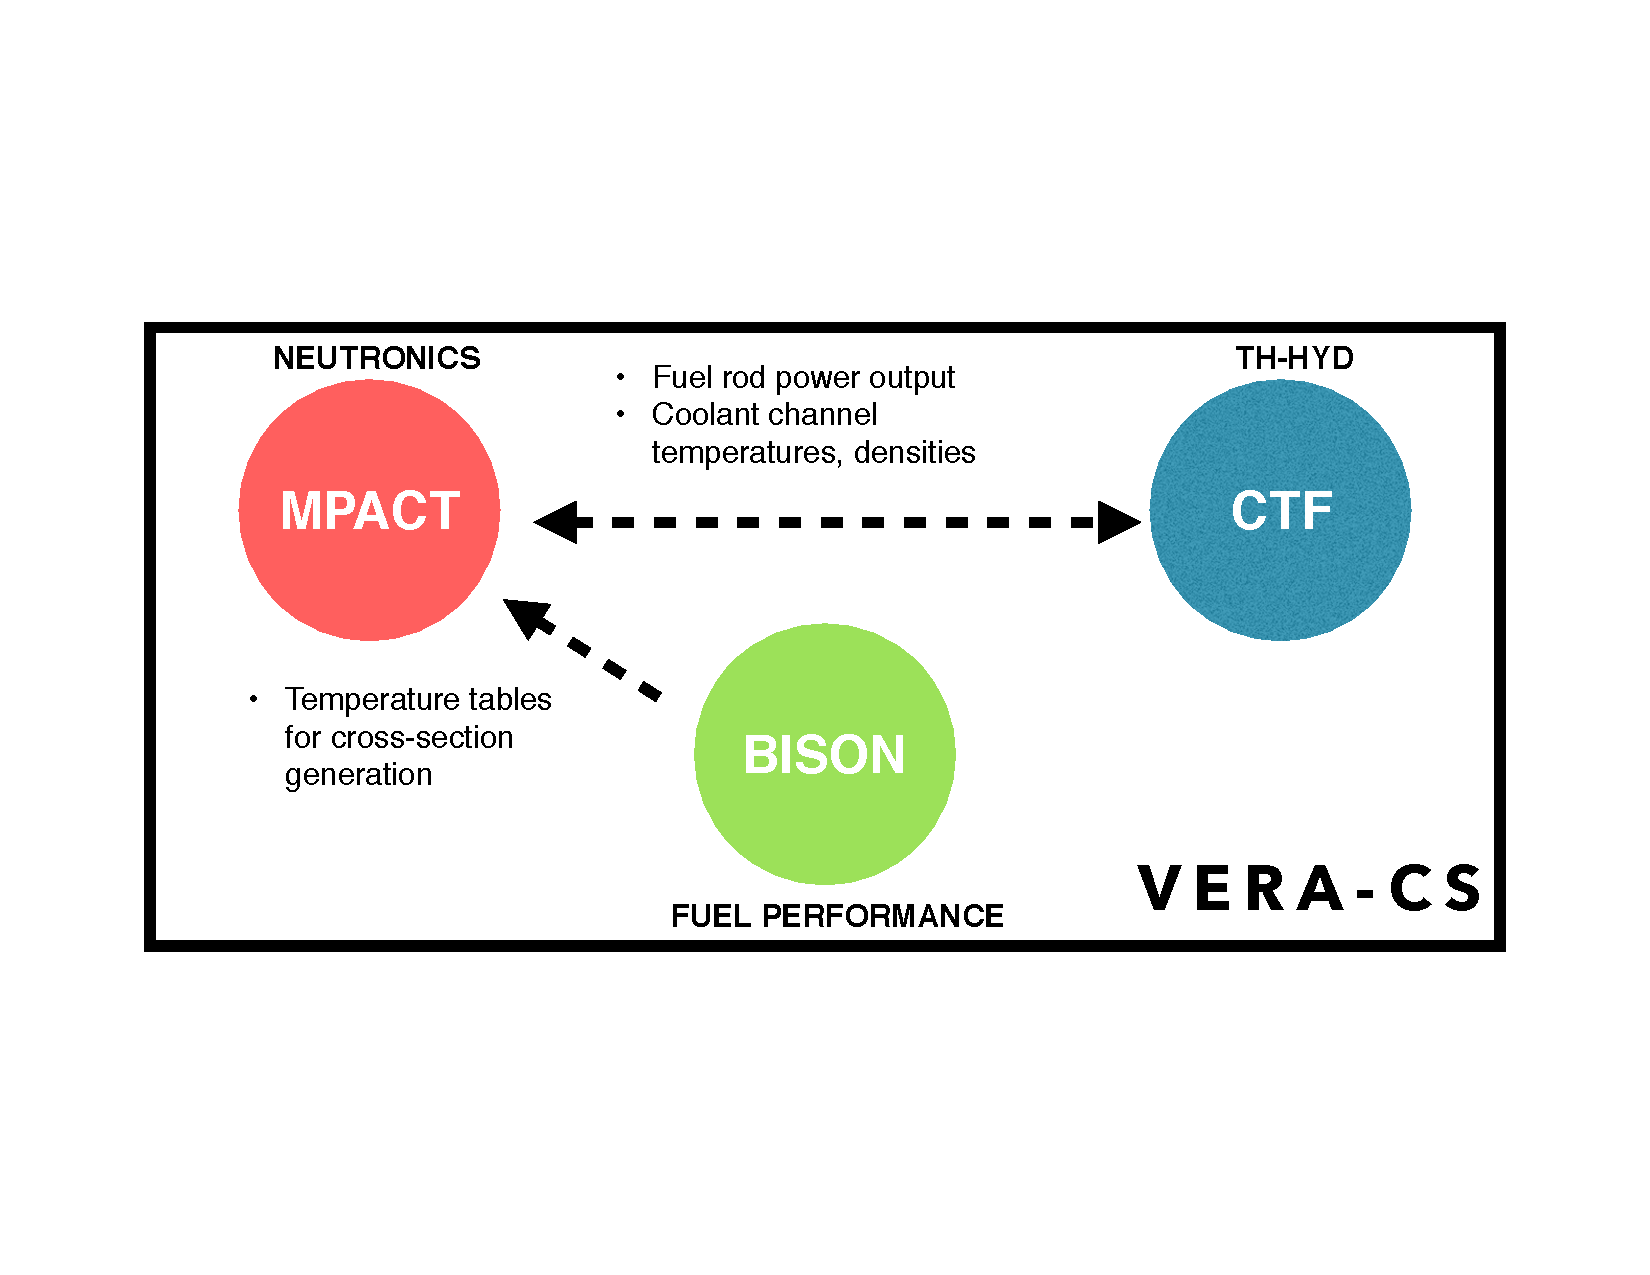
\includegraphics[width=0.5\linewidth,trim={2cm 5cm 2cm 5cm}]{./Figures/VERA-CS-Figure.pdf}
\end{center}
\caption{Primary physics simulator components of VERA-CS used in this work.}
\label{fig:workflow}
\end{figure} 

\subsubsection{MPACT}
MPACT is a neutron transport solver being developed by the \gls{UMich} and \gls{ORNL}. 
It provides pin-resolved flux and power distributions \cite{kochunas_overview_2013}. 
To solve three-dimensional (3D) problems, it employs a 2D/1D method, which decomposes the problem into a 1D axial stack of 2D radial planes \cite{zhu_assessment_2014}. 
These planes are then solved using Method of Characteristics (MOC). 
While there are a variety of axial solvers available, the Nodal Expansion Method (NEM)-simplified P3 (SP3) solver is the default, which wraps a one-node NEM kernel \cite{stimpson_axial_2014}. 
These 2D and 1D solvers are coupled together through transverse leakage to ensure neutron conservation, and they are accelerated using 3D \gls{CMFD}. 

\subsubsection{CTF}
CTF is a subchannel TH code being developed by \gls{ORNL} and \gls{NCSU} for LWR analysis \cite{avramova_ctf:_2009}. 
It simulates two-phase flow with a three-field representation (liquid, droplet, and vapor) assuming the liquid and droplet fields are in a dynamic equilibrium, leaving two energy conservation equations. 
CTF provides significantly higher resolution and physical detail than the internal TH solver in MPACT, thus requires longer execution times. 

\subsubsection{BISON}
The BISON fuel performance code is being developed by \gls{INL} to provide single-rod fuel performance modeling capability to assess best-estimate values of design and safety criteria. 
BISON is able to capture complex thermo-mechanical behavior such as PCI failures in PWRs \cite{montgomery_advanced_2014}. 
%%PCI is controlled by the complex relationship between the mechanical, thermal, and chemical responses of a fuel rod during operation. Consequently, modeling PCI requires an integral fuel performance code to simulate the fundamental processes of these behaviors. 
BISON is built on \gls{INL}'s \gls{MOOSE} package \cite{gaston_moose:_2009}, which uses the finite element method for geometric representation and a Jacobian Free Newton-Krylov (JFNK) scheme to solve systems of partial differential equations \cite{williamson_multidimensional_2012}. 


\subsection{Work Flow and Modeling Strategy}

In the present work, several steps are involved in producing an accurate neutronic/thermal-hydraulics core model. 
Figure \ref{fig:method} displays the VERA-CS modeling stages used in this work.


\begin{figure}
\begin{center}
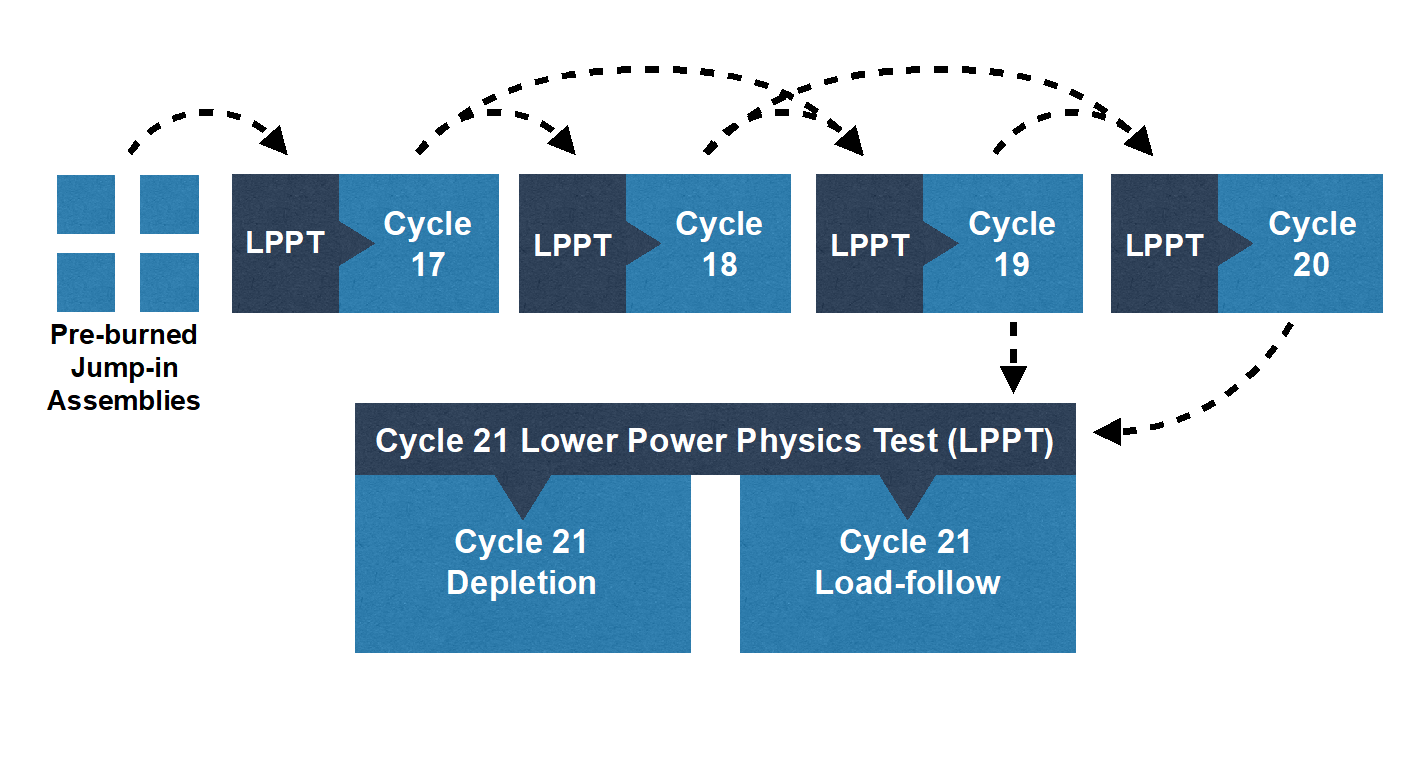
\includegraphics[width=0.5\linewidth]{./Figures/method.png}
\end{center}
\caption{Modeling strategy to simulate load follow in PWR1 cycle 21.}
\label{fig:method}
\end{figure} 

In most cases, each cycle includes assemblies from the previous two cycles, which necessitates a total of five cycles of depletion simulation to provide an accurate isotopic composition and power histories for the oldest assemblies present in cycle 21 (from cycle 19). 
Although it would be most accurate to start modeling from the \gls{BOL} of PWR1, this is computationally impractical. 
In this work, individual pre-burned assemblies were inserted into the cycle 17 core model through a "jump-in" strategy to approximate the shuffled assemblies present in cycle 17 (from cycle 15 and 16). 
These approximate assemblies are removed from the core by the start of cycle 19, which minimizes their effect on isotropic accuracy of our target cycle, cycle 21. 

Because of the difficulties in performing single assembly 3D depletion, special attention was paid to the exposure axial offset of each assembly at its desired burnup. 
During the project it was determined that the exposure axial offset needs to be close to zero to prevent an unrealistic power axial offset from occurring in cycle 17. 
In order to approximate cycle 15 and 16 assemblies as closely as possible, a total of 7 assembly types were burned to 15 target burnups. 
These 15 assemblies were then inserted into the proper position in cycle 17, based on the core loading scheme.


%%%%%%%%%%%%%%%%%%%%%%%%%%%%%%%%%%%%%%%%%%%%%%%%%%%%%%%%%
\section{Summary of Previous Results}
%%%%%%%%%%%%%%%%%%%%%%%%%%%%%%%%%%%%%%%%%%%%%%%%%%%%%%%%%

\subsection{Low Power Physics Testing}
Before the cycle depletion was simulated, a \gls{LPPT} was conducted to validate the shuffling scheme for each cycle, as shown in Figure \ref{fig:method}.
The \gls{LPPT}s included a critical boron search, an \gls{ITC} test and a \gls{CRW} test. 
The \gls{ITC} test was conducted by varying the temperature of the fuel and moderator by $\pm$4 $^\circ$F. 
The change in reactivity was then used to determine the \gls{ITC}. 
The \gls{CRW} tests were performed using a \gls{DRWM} technique, where each control rod bank was individually inserted into the core and the change in reactivity was used to determine the control bank's worth. 
The comparison of the calculated critical boron, \gls{ITC} and \gls{CRW} to their measured value is shown in Table \ref{tab:cb}, and Figure \ref{fig:crw}, respectively. 
It is observed that the MPACT accurately predicts the measured critical boron value from cycle 19 onward.
The \gls{ITC} predictions are within 2 pcm for all cycles, which is within a reasonable margin of error.
In addition, it is observed that the predicted \gls{CRW} values are all within $\pm6$ \%.
It is observed that from cycle 19 onward, the \gls{CRW} values for the different control banks tend to become more irregular.
This irregularity causes the total predicted control rod worth to be within 1 \% for cycle 19, 20 and 21. 
It should be noted that some of the large relative errors observed in the control rod worth comparisons are a results of low measured rod worth. 
Based on these comparisons, it is concluded that any error introduced by the individually burned assemblies inserted into cycle 17 is eliminated by cycle 19, which shows an excellent agreement with the measured values. 
%Additional investigation is required to reduce these errors.   

\begin{table}
\caption{Low Power Physics Results}
\label{tab:cb}
\begin{center}
\begin{tabular}[!t]{|c|c|c|}
\hline
Cycle      & Critical Boron   & Isothermal Temp. Coeff.      \\
           & Difference [ppm] & Difference [pcm/$^{\circ}$F]  \\ \hline
17 & -42 & -0.6     \\\hline
18 & 44  & -1.4     \\\hline
19 & 1   & -1.7     \\\hline
20 & 3 & -0.83     \\\hline
21 & -10 & 0.4     \\\hline
\end{tabular}
\end{center}
\end{table}



\begin{figure}
\begin{center}
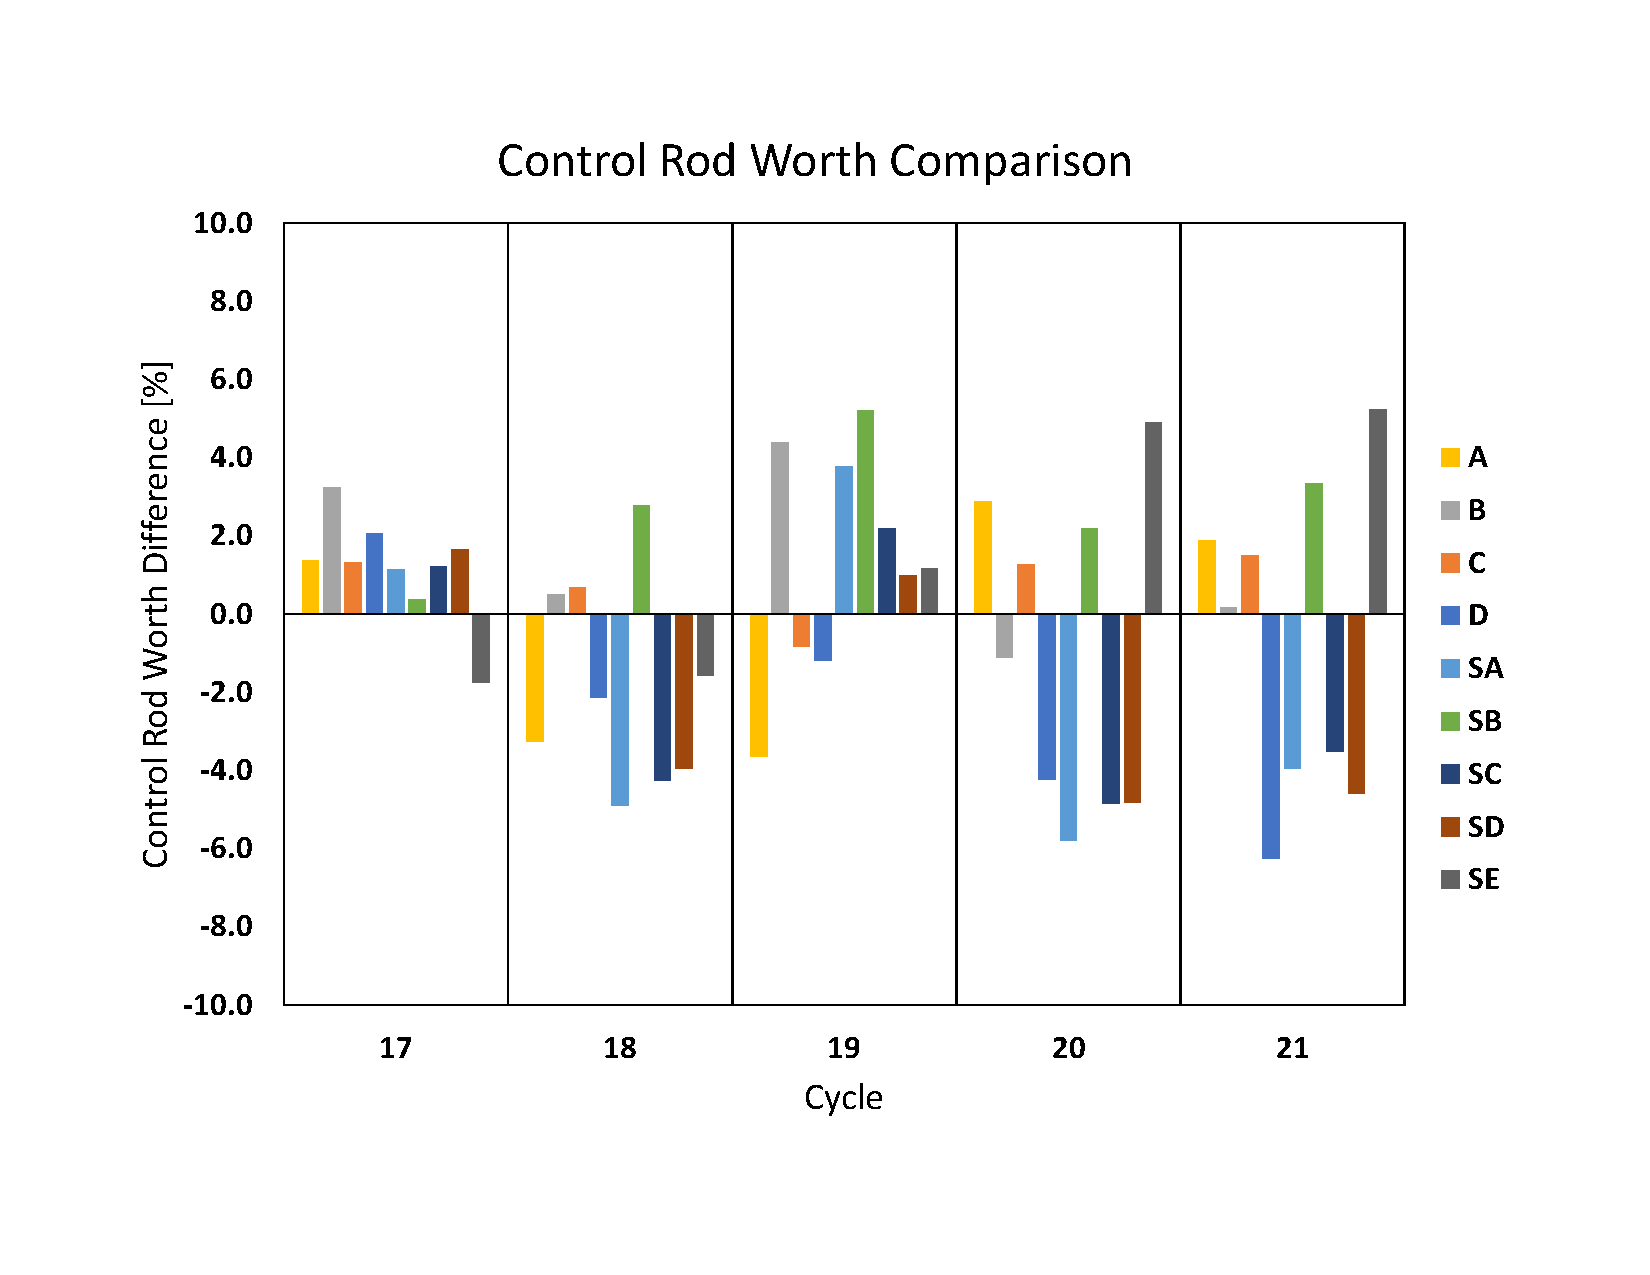
\includegraphics[trim={0 2cm 0 2cm},clip,width=0.5\linewidth]{./Figures/crw_diff.pdf}
\end{center}
\caption{Comparison of control rod worth of all 9 rod banks at HZP.}
\label{fig:crw}
\end{figure} 

\subsection{Cycle Depletion}
After the shuffling scheme for each cycle had been validated, cycle depletion was simulated from the \gls{BOC} to the \gls{EOC}, with special attention paid to the shutdown time between \gls{EOC} and \gls{BOC} of the next cycle to ensure accurate fission product decay between cycles. 
As the fuel is depleted over a reactor cycle, the boron concentration in the coolant is reduced via dilution to maintain criticality. 
In addition to the boron concentration being diluted over the length of the cycle, the weight percent of $^{10}$B is also reduced. 
This reduction is a result of boron depletion and is known to increase the critical boron concentration during the later dates of the cycle. 
MPACT can account for boron depletion through explicit input of $^{10}$B enrichment, but this requires measurements of the $^{10}$B concentration before the simulation can be performed.
As an alternative, the simulations is conducted with a constant $^{10}$B enrichment of 19.9 w/o and the measured critical boron is corrected using the measured $^{10}$B enrichment.
\begin{figure}
\begin{center}
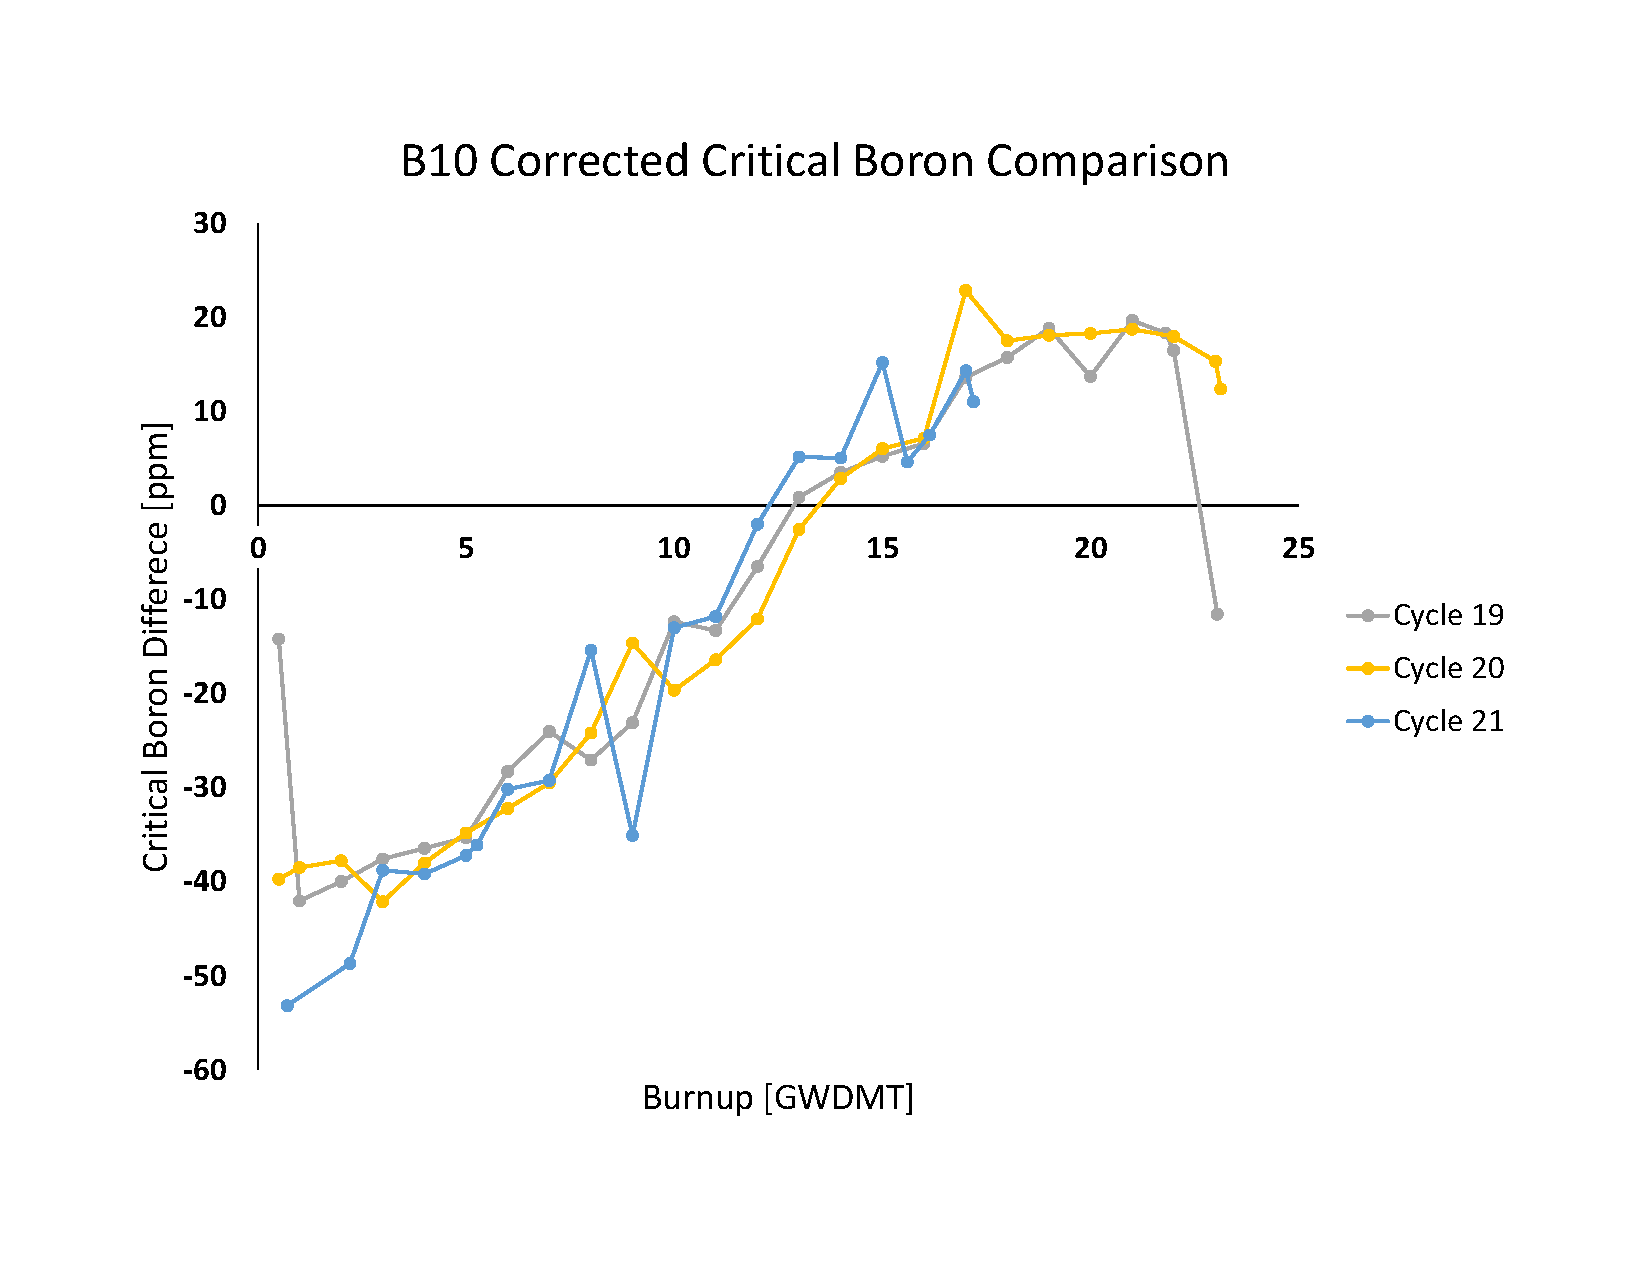
\includegraphics[trim={0 2cm 0 3.1cm},clip,width=0.5\linewidth]{./Figures/corr_b.pdf}
\end{center}
\caption{Comparison of simulated to the measured critical boron concentrations.}
\label{fig:cor_b}
\end{figure} 

The measured boron concentrations were used to establish the accuracy of the core reactivity vs. fuel burnup. 
The boron "letdown" is compared for cycles 19-21 in Figure \ref{fig:cor_b}. 
Figure \ref{fig:cor_b} contains a comparison of the corrected measured boron concentration with the MPACT simulation. 
%This correction accounts for the depletion of $^{10}$B over the length of the cycle by scaling the measured boron concentration with the ratio of the the measured $^{10}$B concentration to the MPACT $^{10}$B concentration.
As shown in Figure \ref{fig:cor_b}, the difference between corrected measured and simulated critical boron concentration varies between -40 ppm at the beginning of cycle to +20 ppm at the end of the cycle. 
The cause of this reactivity swing is believed to be the temperature tables used to determine the fuel's temperature as a function of burnup and linear heat rate.
These tables are not used during \gls{HZP} calculations, which show good agreement to the measured values, and are constant for all three cycles, which have very consistent discrepancies.
Regardless, the difference is within 50 ppm for each cycle depletion, which is considered sufficiently accurate.



%%%%%%%%%%%%%%%%%%%%%%%%%%%%%%%%%%%%%%%%%%%%%%%%%%%%%%%%%
\section{Load-Follow Operation}
%%%%%%%%%%%%%%%%%%%%%%%%%%%%%%%%%%%%%%%%%%%%%%%%%%%%%%%%%

%%%%%%%%%%%%%%%%%%%%%%%%%%%%%%%%%%%%%%%%%%%%%%%%%%%%%%%%%
%%%%%%%%%%%%%%%%%%%%%%%%%%%%%%%%%%%%%%%%%%%%%%%%%%%%%%%%%
\chapter{Methodology}
%%%%%%%%%%%%%%%%%%%%%%%%%%%%%%%%%%%%%%%%%%%%%%%%%%%%%%%%%
%%%%%%%%%%%%%%%%%%%%%%%%%%%%%%%%%%%%%%%%%%%%%%%%%%%%%%%%%

%%%%%%%%%%%%%%%%%%%%%%%%%%%%%%%%%%%%%%%%%%%%%%%%%%%%%%%%%
\section{BISON}
%%%%%%%%%%%%%%%%%%%%%%%%%%%%%%%%%%%%%%%%%%%%%%%%%%%%%%%%%

%%%%%%%%%%%%%%%%%%%%%%%%%%%%%%%%%%%%%%%%%%%%%%%%%%%%%%%%%
\section{MPACT Screening Process}
%%%%%%%%%%%%%%%%%%%%%%%%%%%%%%%%%%%%%%%%%%%%%%%%%%%%%%%%%

%%%%%%%%%%%%%%%%%%%%%%%%%%%%%%%%%%%%%%%%%%%%%%%%%%%%%%%%%
%%%%%%%%%%%%%%%%%%%%%%%%%%%%%%%%%%%%%%%%%%%%%%%%%%%%%%%%%
\chapter{Results and Discussion}
%%%%%%%%%%%%%%%%%%%%%%%%%%%%%%%%%%%%%%%%%%%%%%%%%%%%%%%%%
%%%%%%%%%%%%%%%%%%%%%%%%%%%%%%%%%%%%%%%%%%%%%%%%%%%%%%%%%

%%%%%%%%%%%%%%%%%%%%%%%%%%%%%%%%%%%%%%%%%%%%%%%%%%%%%%%%%
\section{BISON}
%%%%%%%%%%%%%%%%%%%%%%%%%%%%%%%%%%%%%%%%%%%%%%%%%%%%%%%%%

%%%%%%%%%%%%%%%%%%%%%%%%%%%%%%%%%%%%%%%%%%%%%%%%%%%%%%%%%
\section{Limiting Pin}
%%%%%%%%%%%%%%%%%%%%%%%%%%%%%%%%%%%%%%%%%%%%%%%%%%%%%%%%%

%%%%%%%%%%%%%%%%%%%%%%%%%%%%%%%%%%%%%%%%%%%%%%%%%%%%%%%%%
%%%%%%%%%%%%%%%%%%%%%%%%%%%%%%%%%%%%%%%%%%%%%%%%%%%%%%%%%
\chapter{Conclusions}
%%%%%%%%%%%%%%%%%%%%%%%%%%%%%%%%%%%%%%%%%%%%%%%%%%%%%%%%%
%%%%%%%%%%%%%%%%%%%%%%%%%%%%%%%%%%%%%%%%%%%%%%%%%%%%%%%%%

We conclude that graduate students like coffee.

\backmatter
\bibliographystyle{ans}
\bibliography{Masters}

\chapter{Vita}

Juan Valdez was born\ldots.

\end{document}
\endinput
%%
%% End of file `thesis-ex.tex'.
